\documentclass[a4paper]{article}
\usepackage[top=1in, bottom=1.25in, left=1.25in, right=1.25in]{geometry}
\usepackage{amsmath}
\usepackage{multicol}
\usepackage{graphicx}
\usepackage{subfig}

%\RequirePackage{ltxcmds}[2010/12/07]
%opening
\title{Linear Filtering in Frequency-Domain}
\author{ }
\date{ }
\begin{document}

\maketitle
\section{Introduction}
Linear filtering can be easily implemented in time-domain resorting to the use of finite impulse response (FIR) digital filters and convolution property as,
\begin{equation}
    y(n)= \sum\limits_{k=0}^{N-1} x(n-k)h\left(k\right),
    \label{genFIR}
\end{equation}
where $x(n)$ is the input signal, $h(k)$ is a length-$N$ sequence filter coefficients, $y(n)$ represents the filtered output signal and $N$ is the number of filter coefficients.
Analysing this equation we can note that, for a block signal of length $N$, the required number of operations for the direct calculation of equation~\eqref{genFIR} evolves with $N^2$, $\mathcal{O}(N^2)$. This limitation imposed the emergence of algorithm, where the linear convolution is calculated faster than directly implementing \eqref{genFIR}.
In this sense, fast convolution can be implemented by sectioning or block the signal and use the fast Fourier transform (FFT)/ inverse fast Fourier transform (IFFT) on these blocks to take advantage of the efficiency of the FFT. However, the implementation of non-cyclic convolution with the finite-length of cyclic convolution that the FFT provides needs to be fixed. A solution to this problem was achieved through the application of overlap-save and overlap-add method, where the complexity evolves in log scale $\mathcal{O}(N\log_2N)$. The general method is to split the input signal into manageable blocks, then apply the FFT to to perform the linear convolution and at the end recombine the output blocks such that it is avoided the wrap-around errors.

\section{Overlap-Save Method}
In this method we start by adding R null samples at the beginning of the sequence, which is commonly equal to the length of the impulse response of the filter. Then, the data is divided into blocks of length $N$ samples, but with successive blocks overlapping by $R$ samples.
Then, the an $N$-point FFT is computed for each data block. Then, the multiplication of $N$-point FFT and the transfer function is performed, followed by IFFT operations to obtain the time-domain block signal. These initial samples are then discarded, and only the error-free $N-R$ samples are saved in the output record.
In the figure below is illustrated an example of overlap-add method with $R=\frac{N}{2}$ and $L=N-R=R$.

\subsection{Frequency Response of Filter}
\begin{figure*}[h!]
    \centering
    \subfloat[]{{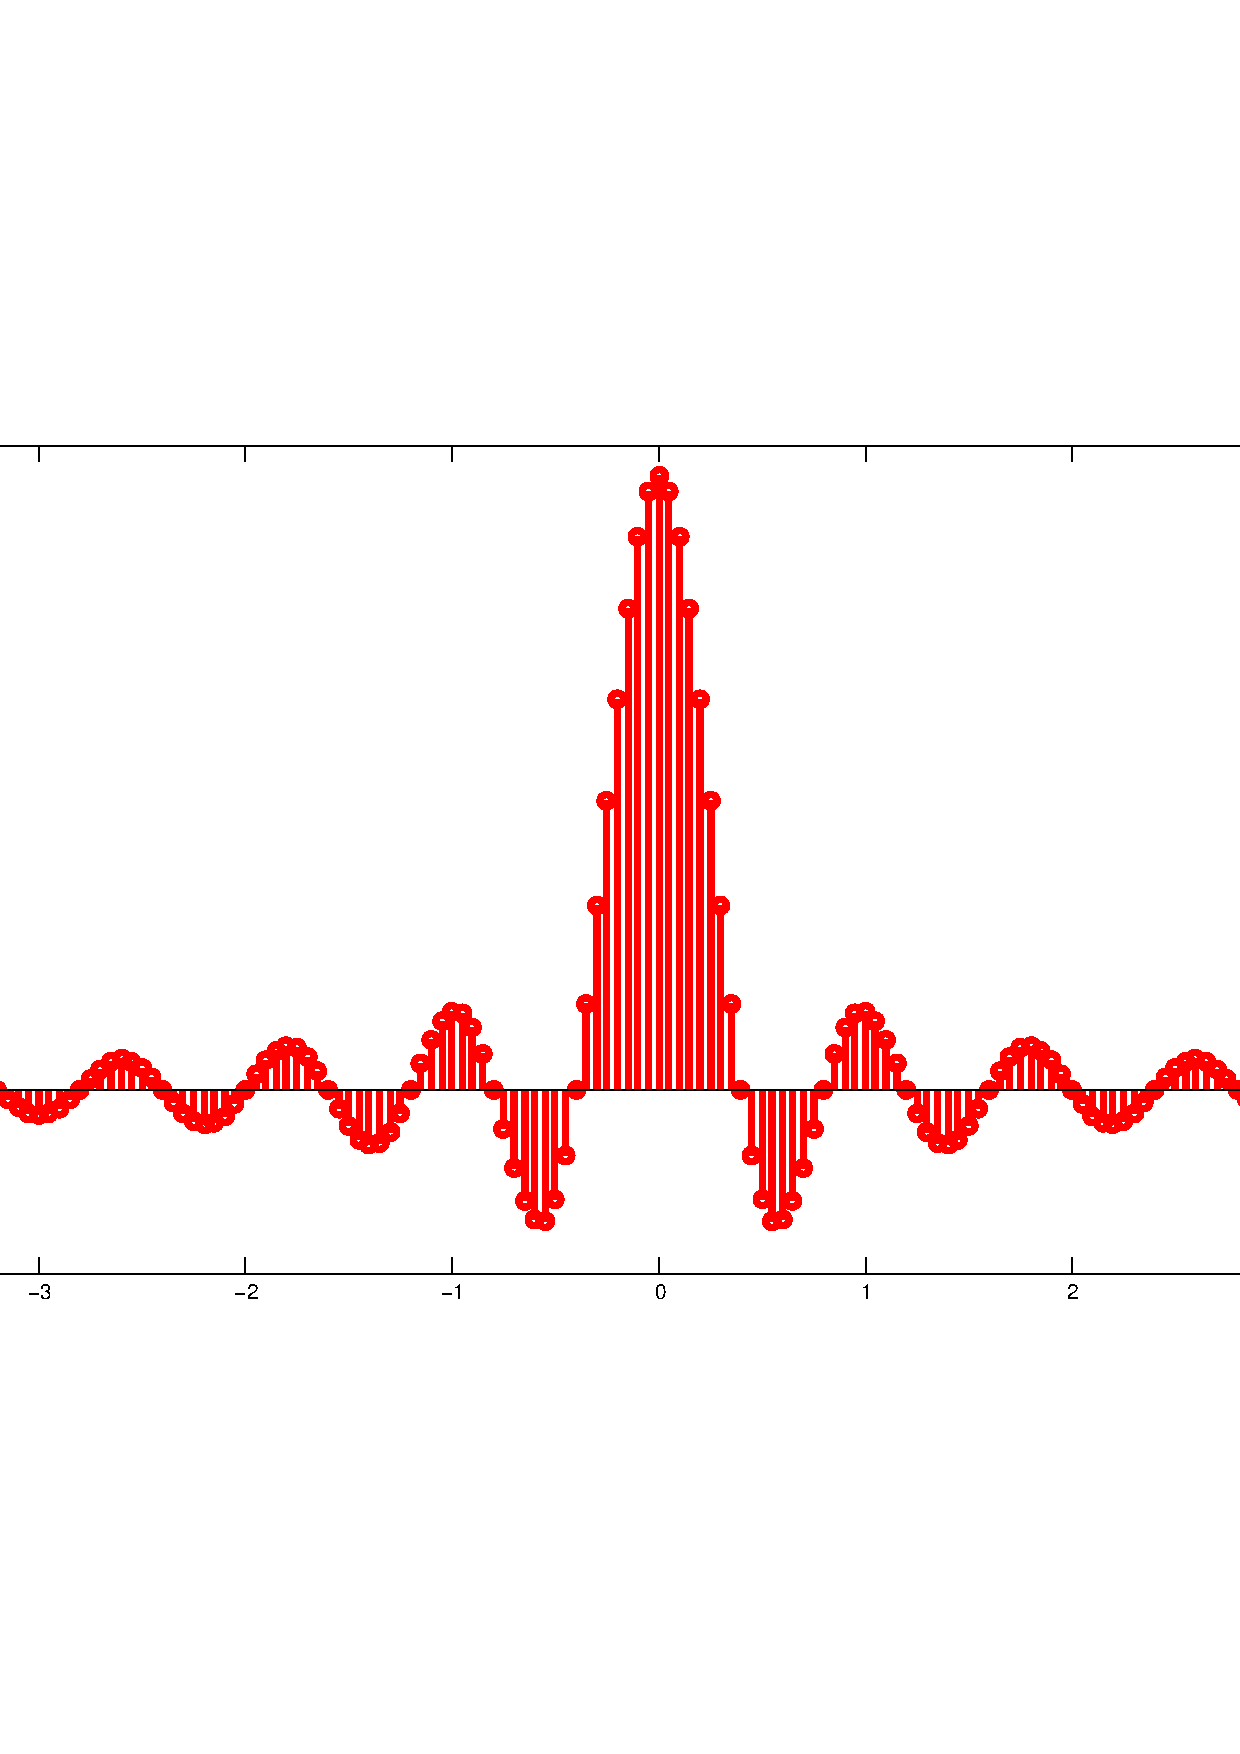
\includegraphics[width=.46\linewidth]{rc-td-filter-stem} }}%
    \qquad
    \subfloat[]{{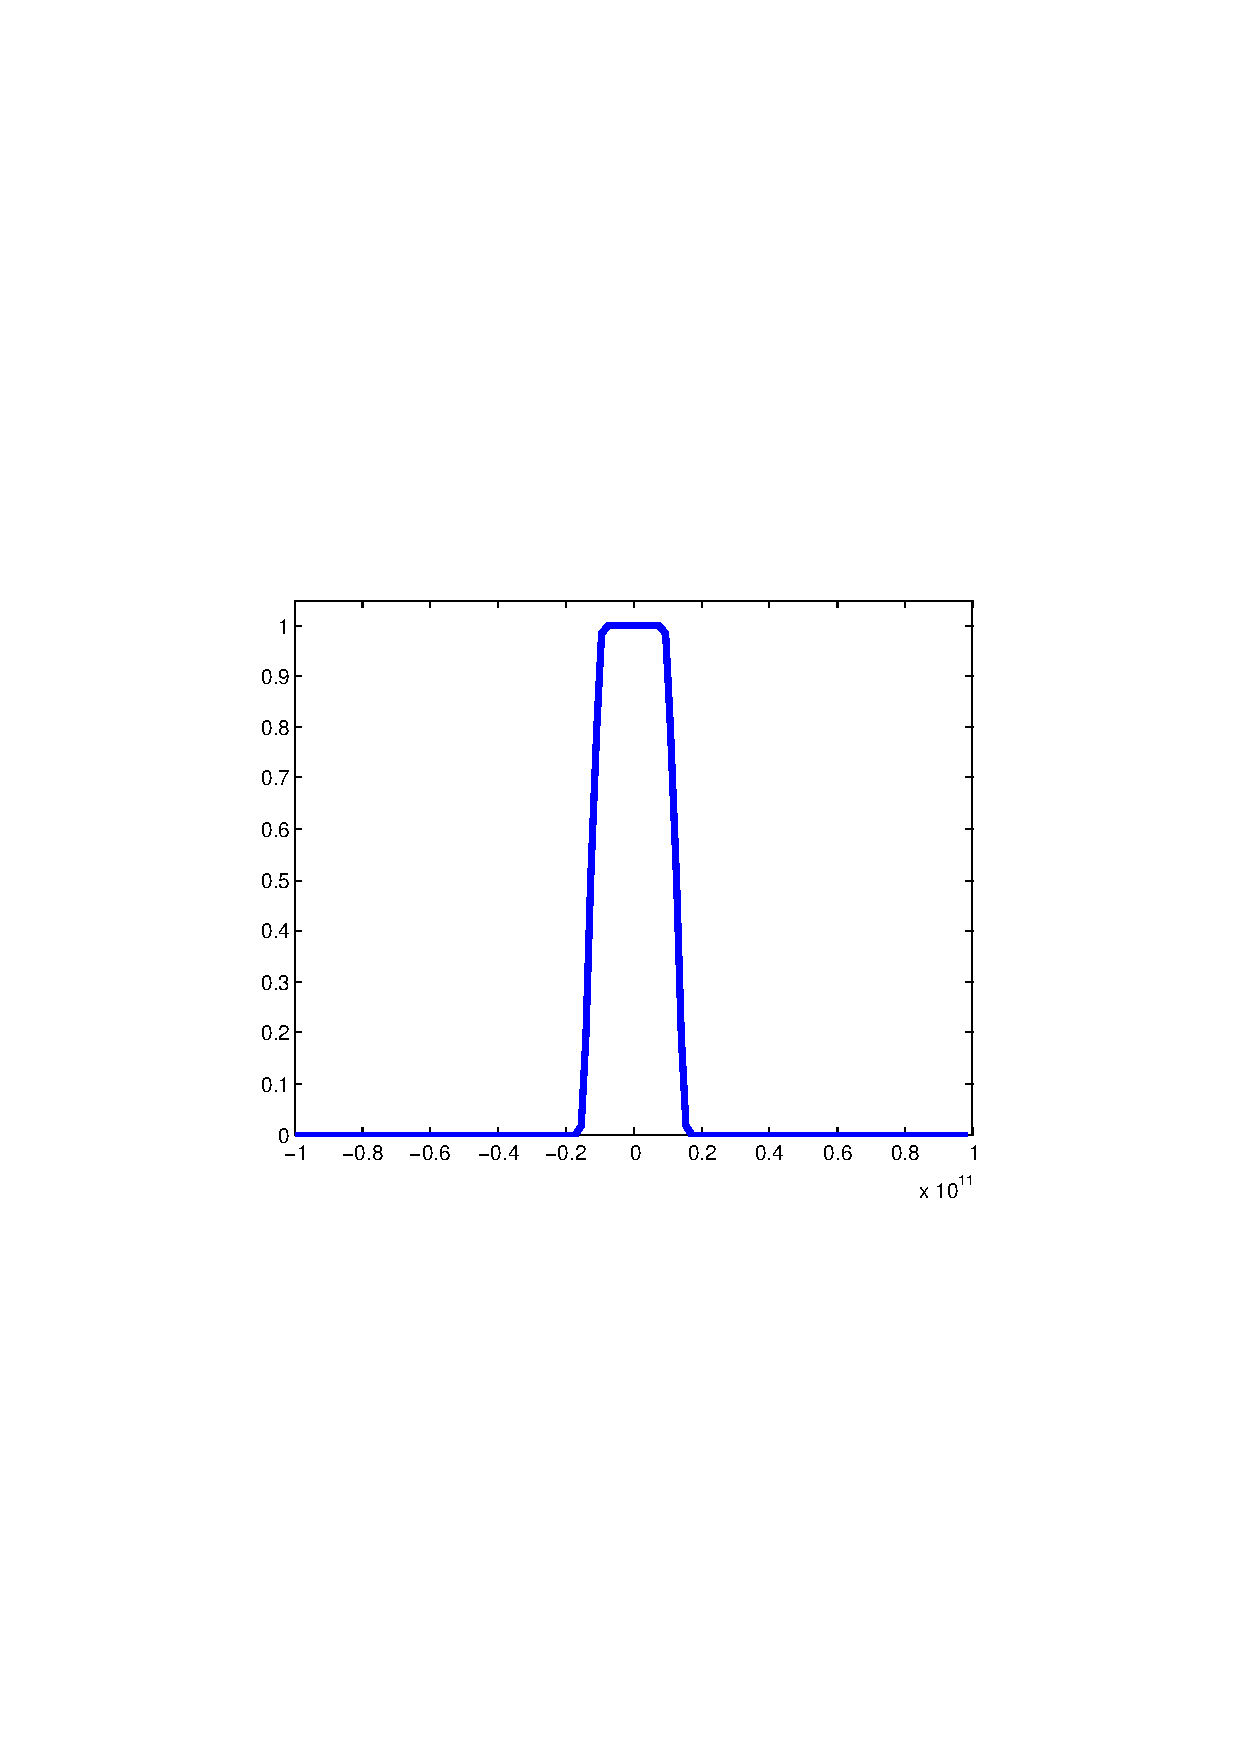
\includegraphics[width=.46\linewidth]{rc-fd-filter-SpS8} }}%
    \caption{ a) Impulse response of raised cosine filter; b) Frequency response  of raised cosine filter. }%
    \label{BER_InputPower}%
\end{figure*}
An example of FIR filter (\textit{raised-cosine filter}) is presented in Fig. 1, including its impulse response, $h(k)$, and frequency response, $H(f)$. The frequency response of filter can be obtained from the FFT of impulse response of the filter.
By performing the FFT operation on $h(k)$, the frequency response of the filter will be limited to the frequency interval, [$-\frac{F_s}{2}$, $\frac{F_s}{2}$], and this range show us the $N$ frequency components obtained from FFT. The minimum frequency bin is $-\frac{F_s}{2}$ and the maximum bin is $\frac{F_s}{2}$, in which $F_s$ corresponds to the sampling frequency. We can note that the spectral width of $H(f)$ is $F_s$, which is the inverse of sampling period, $T_s$. It is also important to note that, for a given sampling frequency, the frequency resolution, $\Delta R$, of $H(f)$ depends on the parameter $N$ and it increases with $N$, $\Delta R=\frac{F_s}{N}$.
\begin{figure}[h]
    \centering
    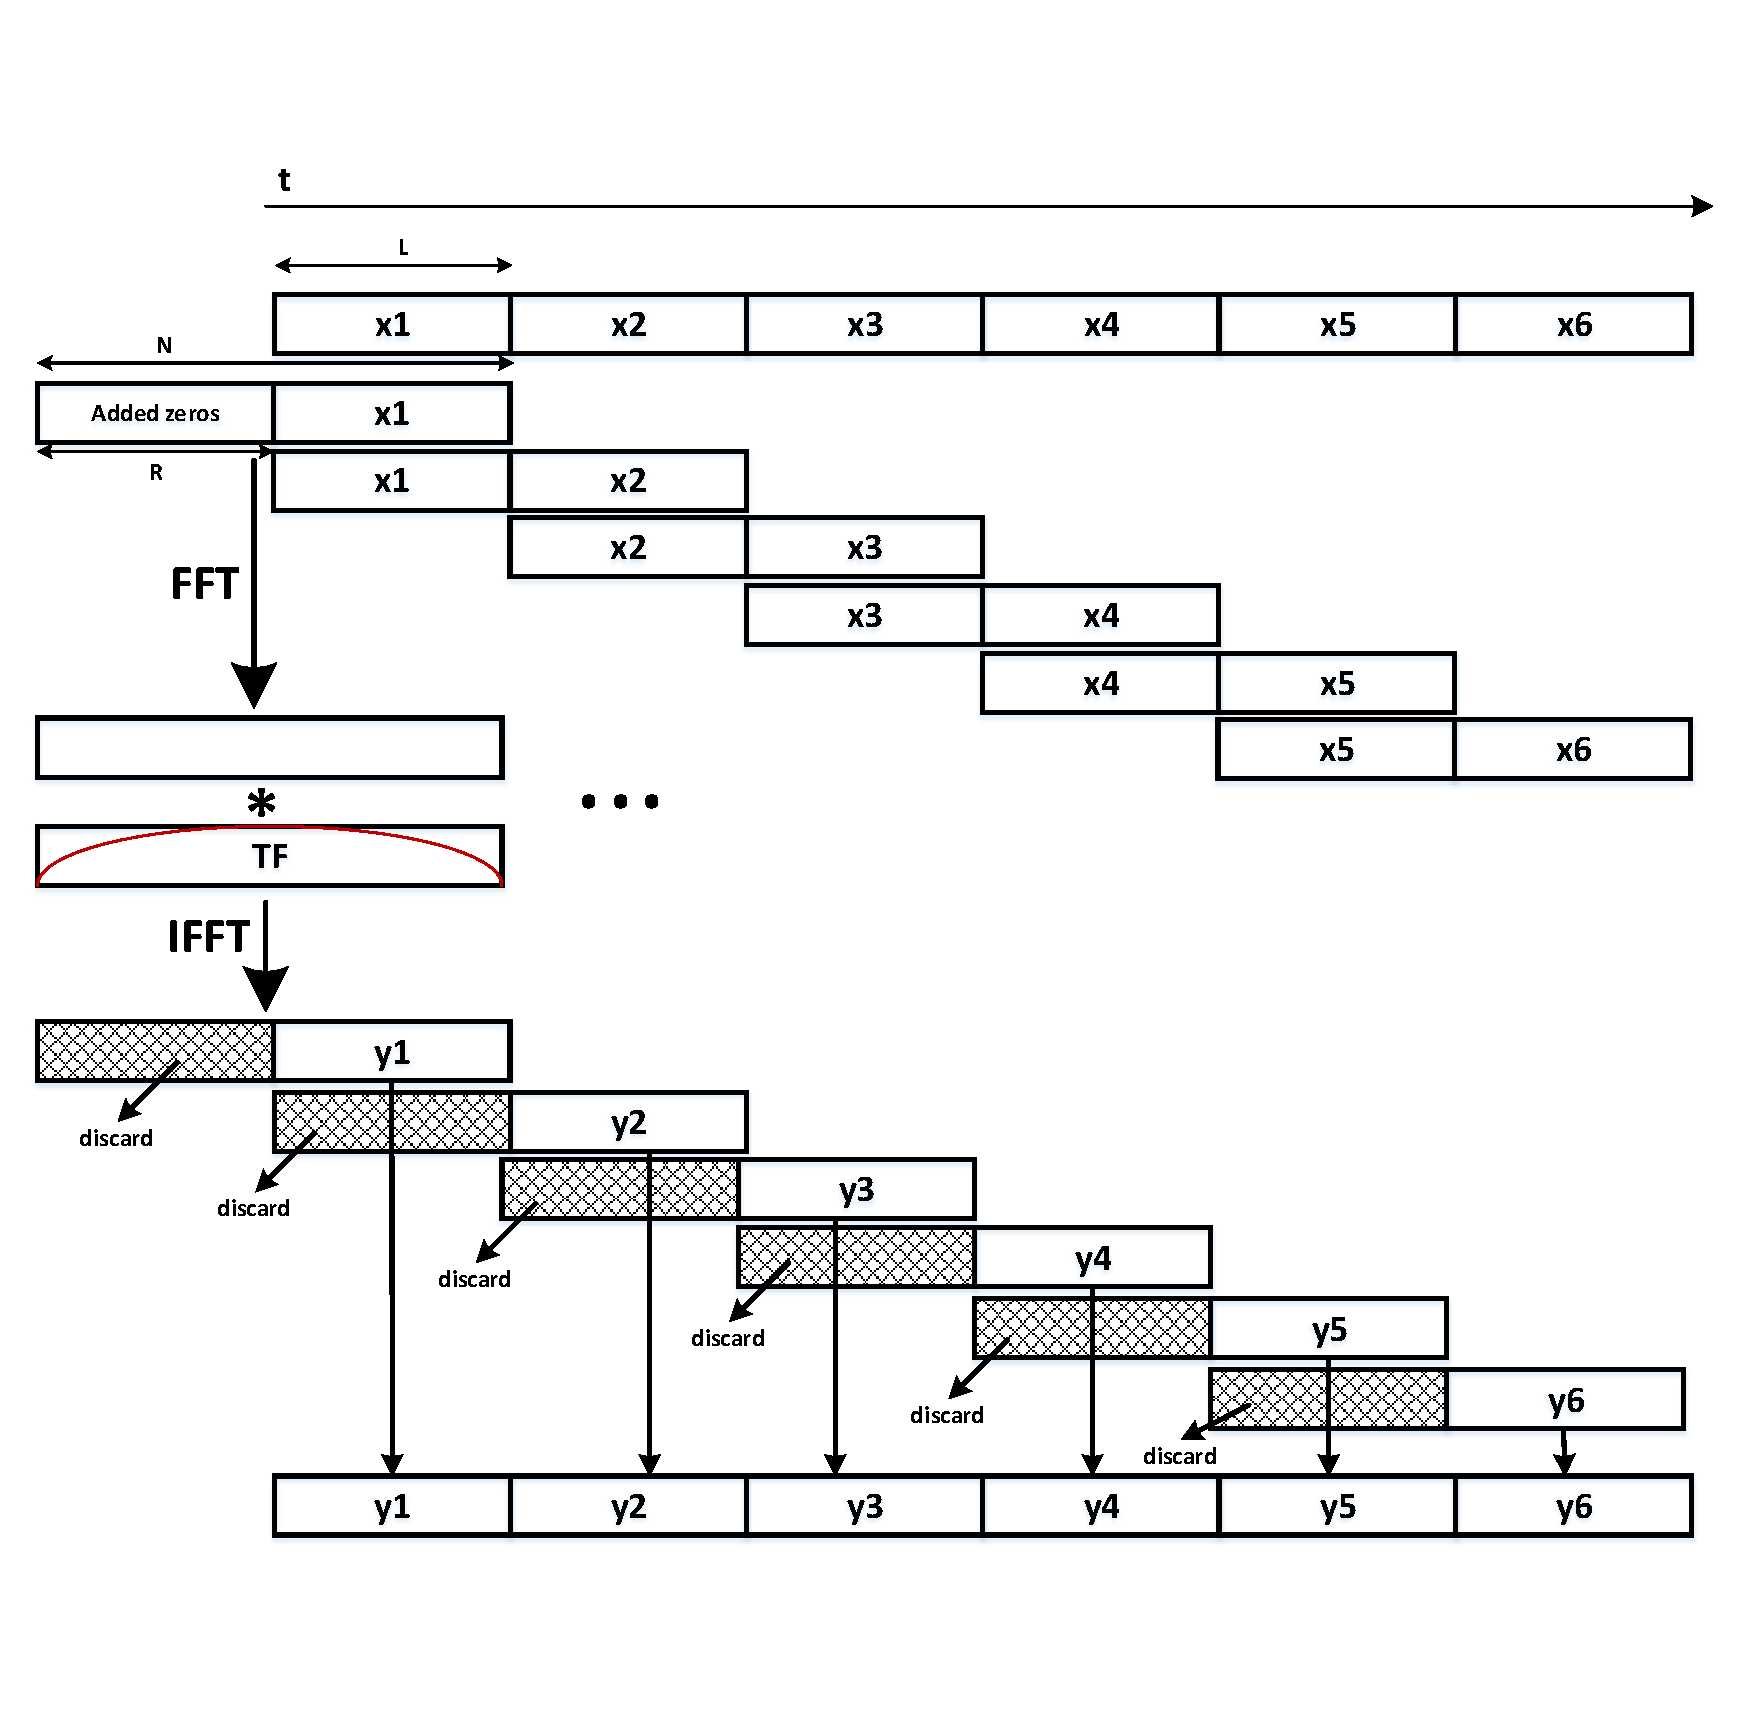
\includegraphics[width=15cm]{overlap-savev2}
\end{figure}

\end{document} 